\documentclass[conference]{IEEEtran}
\usepackage{savesym}
\usepackage{amsmath,amssymb,amsfonts,amsthm}
\usepackage[numbers]{natbib}
\usepackage{algorithm}
\usepackage[noend]{algpseudocode}
\usepackage{comment}
\usepackage{xspace}
\usepackage{scalerel}
\usepackage{xcolor}
\usepackage[caption=false,font=footnotesize]{subfig}
\usepackage[left]{showlabels}
\usepackage{multicol}
\usepackage[bookmarks=true]{hyperref}

\begin{document}

\title{	Online, interactive user guidance for \\
		high-dimensional, constrained motion planning }

\author{Fahad Islam, Oren Salzman and Maxim Likhachev}


\maketitle
\thispagestyle{empty}
\pagestyle{empty}

\def\frechet{Fr\'echet\xspace}

\newcommand{\cupdot}{\mathbin{\mathaccent\cdot\cup}}

%unlabeled PSPACE-hardness paper
\newcommand{\mtm}{\emph{multi-to-multi}\xspace}
\newcommand{\mts}{\emph{multi-to-single}\xspace}
\newcommand{\sts}{\emph{multi-to-single-restricted}\xspace}
\newcommand{\dtd}{\emph{single-to-single}\xspace}

\newcommand{\cte}{\emph{full-to-edge}\xspace}
\newcommand{\ctc}{\emph{full-to-full}\xspace}
\newcommand{\ete}{\emph{edge-to-edge}\xspace}

\newcommand{\AND}{{\sc and}\xspace}
\newcommand{\OR}{{\sc or}\xspace}

%tex tools
\newcommand{\ignore}[1]{}

%%% algorithms
\def\vor{\text{Vor}}

\def\P{\mathcal{P}} \def\C{\mathcal{C}} \def\H{\mathcal{H}}
\def\F{\mathcal{F}} \def\U{\mathcal{U}} \def\L{\mathcal{L}}
\def\O{\mathcal{O}} \def\I{\mathcal{I}} \def\E{\mathcal{E}}
\def\S{\mathcal{S}} \def\G{\mathcal{G}} \def\Q{\mathcal{Q}}
\def\I{\mathcal{I}} \def\T{\mathcal{T}} \def\L{\mathcal{L}}
\def\N{\mathcal{N}} \def\V{\mathcal{V}} \def\B{\mathcal{B}}
\def\D{\mathcal{D}} \def\W{\mathcal{W}} \def\R{\mathcal{R}}
\def\M{\mathcal{M}} \def\X{\mathcal{X}} \def\A{\mathcal{A}}
\def\Y{\mathcal{Y}} \def\L{\mathcal{L}}

\def\dS{\mathbb{S}} \def\dT{\mathbb{T}} \def\dC{\mathbb{C}}
\def\dG{\mathbb{G}} \def\dD{\mathbb{D}} \def\dV{\mathbb{V}}
\def\dH{\mathbb{H}} \def\dN{\mathbb{N}} \def\dE{\mathbb{E}}
\def\dR{\mathbb{R}} \def\dM{\mathbb{M}} \def\dm{\mathbb{m}}
\def\dB{\mathbb{B}} \def\dI{\mathbb{I}} \def\dM{\mathbb{M}}

\def\eps{\varepsilon}
\def\obs{\mathrm{obs}}

\newcommand{\sbs}{sampling-based\xspace}
\newcommand{\mr}{multi-robot\xspace}
\newcommand{\mpl}{motion planning\xspace}
\newcommand{\cs}{configuration space\xspace}
\newcommand{\conf}{configuration\xspace}
\newcommand{\confs}{configurations\xspace}
\newcommand{\etal}{et al.\xspace}

% programming
\newcommand{\Cpp}{C\raise.08ex\hbox{\tt ++}\xspace}



\newcommand{\ch}{\mathrm{ch}}
\newcommand{\pspace}{{\sc pspace}\xspace}
\newcommand{\np}{{\sc np}\xspace}
\newcommand{\degree}{\ensuremath{^\circ}}
\newcommand{\argmin}{\operatornamewithlimits{argmin}}


\newcommand{\dist}{\textup{dist}}

\newcommand{\Cfree}{\C_{\textup{free}}}
\newcommand{\Cforb}{\C_{\textup{forb}}}

\newtheorem{lemma}{Lemma}
\newtheorem{theorem}{Theorem}
\newtheorem{corollary}{Corollary}
\newtheorem{claim}{Claim}

\newtheorem{definition}{Definition}
\newtheorem{remark}{Remark}
\newtheorem{observation}{Observation}

\def\os#1{\textcolor{blue}{#1}}
\def\ToDo#1{\textcolor{magenta}{\textbf{ToDo:}~#1}}


\makeatletter
\def\thmhead@plain#1#2#3{%
  \thmname{#1}\thmnumber{\@ifnotempty{#1}{ }\@upn{#2}}%
  \thmnote{ {\the\thm@notefont#3}}}
\let\thmhead\thmhead@plain
\makeatother

\def\todo#1{\textcolor{blue}{\textbf{TODO:} #1}}
\def\new#1{\textcolor{magenta}{#1}}
\def\old#1{\textcolor{red}{#1}}

\def\removed#1{\textcolor{green}{#1}}
%\def\removed#1{}
%%% Local Variables:
%%% mode: plain-tex
%%% TeX-master: "main"
%%% End:
\algrenewcommand\textproc{}

\newcommand\algname[1]{\textsf{#1}\xspace}
\newcommand\astar{\algname{A*}}
\newcommand\mhastar{\algname{MHA*}}

\newcommand{\arxiv}[2]{#1}

\begin{abstract}
We consider the problem of planning a collision-free path for a high-dimensional robot.
Specifically, we suggest a planning framework where a motion-planning algorithm can obtain guidance from a user.
In contrast to existing approaches, we suggest to seek user guidance only when the planner identifies that it is in a local minimum, namely when it ceases to make significant progress towards the goal.
User guidance is given in the form of an intermediate configuration $\hat{q}$ which, in turn, is used to bias the planner to go through $\hat{q}$.
We demonstrate our approach for the case where the planning algorithm is Multi-Heuristic A* (MHA*) and the robot is a 34-DOF humanoid.
\end{abstract}

\IEEEpeerreviewmaketitle

%%%%%%%%%%%%%%%%%%%%%%%%%%%%%%%%%%%%%%%%%%%%%%%%%%%%%
%Intro
%%%%%%%%%%%%%%%%%%%%%%%%%%%%%%%%%%%%%%%%%%%%%%%%%%%%%
%\begin{comment}
\section{Introduction}
\label{sec:intro}

Motion-planning is a fundamental problem in robotics that has been studied for over four decades. 
However, efficiently planning paths in high-dimensional, constrained spaces remains an ongoing challenge.
One approach to address this challenge is to incorporate user guidance.
While there has been much work on planning using human demonstration 
(see, e.g.,~\cite{HS16, PHCL16, SHLA16, YA17}), 
%(see, e.g.,~\cite{SHLA16, YA17} for a partial list), 
there has been far less research incorporating guidance as an interactive part of the planning~loop.

Broadly speaking, interactive planning has been typically used in the context of sampling-based motion-planning algorithms~\cite{L06}.
User guidance was employed by biasing the sampling scheme of the planner.
This was done by having the user mark regions in the \emph{workspace} that should be avoided or 
explored~\cite{DSJA14}.
%explored~\cite{DSJA14, MTMKDC15, YPB15}.
Alternatively interactive devices such as a 3D mouse or a haptic arm have been used to generate paths in a (low-dimensional) configuration space. This path was then used by a planner to bias its 
%sampling domain~\cite{TFF12}.
sampling domain~\cite{BTFF16, FTF09, TFF12}.
%Interestingly, in all the examples mentioned, an implicit assumption taken is that the user is dedicated to guide and interact with the planning algorithm.

We are interested in planning in high-dimensional, constrained spaces such as those encountered by a humanoid robot (see Fig.~\ref{fig:robot}).
In such settings, workspace regions often give little guidance to the planner due to the dimension of the configuration space as well as the physical constraints of the robot.
Similarly, obtaining user guidance in the configuration space is extremely time consuming, even for expert users.


Thus,  while beneficial, user guidance should be employed scarcely.
Our key insight is that carefully chosen individual configurations suggested by a user can be used to effectively guide the planner when in need of guidance.


Transforming this insight into a planning framework requires addressing three fundamental questions:

\begin{itemize}
	\item[\textbf{Q1.}] When should the planner ask the user for guidance?
	\item[\textbf{Q2.}] What form should the user's guidance take?
	\item[\textbf{Q3.}] How should the guidance be used?
\end{itemize}
 
In the following, we detail our planning framework (Sec.~\ref{sec:high}) and how it addresses each of these questions (Sec.~\ref{sec:q1}-\ref{sec:q3}).
We then continue (Sec.~\ref{sec:eval}) to demonstrate its effectiveness in simulations and conclude by describing possible additional future work.

\begin{figure}[tb]
  \centering
  	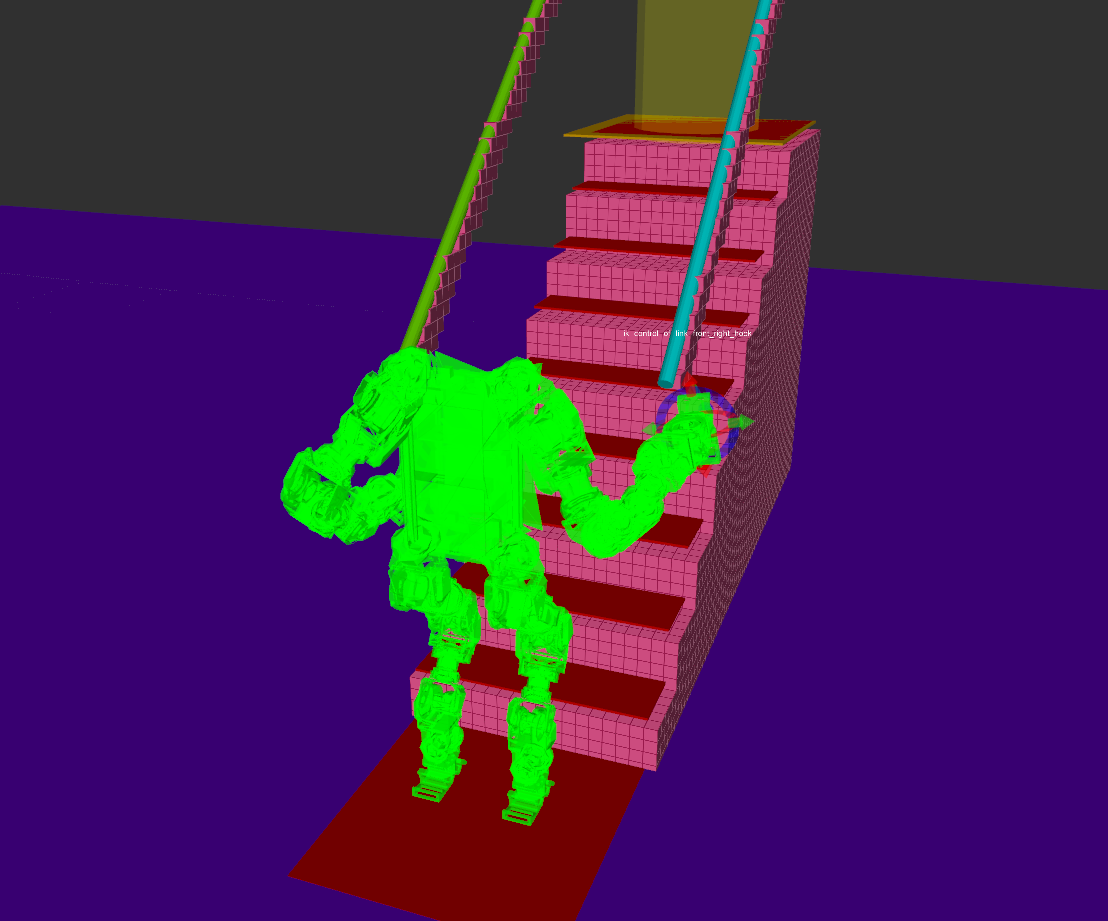
\includegraphics[width=0.283\textwidth]{workspace.png}
  	\vspace{-2mm}
  \caption{
		Planning domain---Humanoid robot needs to climb the stairs while avoiding collision with the obstacles and while adhering to the physical stability constraints.
  	}
   	\label{fig:robot}
\end{figure}

%\algrenewcommand\algorithmicindent{.8em}
\begin{algorithm}[tb]
\caption{Planning framework ($\A$)}
\label{alg:main}	
\begin{algorithmic}[1]
\small
\While{$\neg\A.$\texttt{is\_solution\_found()} } 
	\While{$\neg\A.$\texttt{is\_in\_local\_minima()}} 
		\State $\A.$\texttt{run()}
		\Comment{no user guidance}
	\EndWhile
	
	\State {$g \leftarrow$ \texttt{get\_user\_guidance()}}
	\Comment{$\A$ is in a local minima}
	\State $\A.$\texttt{update\_user\_guidance($g$)}
	\Comment{account for guidance}
	\While{$\A.$\texttt{is\_in\_local\_minima()}}
		\State $\A.$\texttt{run()}
		\Comment{planner uses guidance}
	\EndWhile

	\State $\A.$\texttt{update\_user\_guidance($\neg g$)}
	\Comment {remove  guidance}
\EndWhile
\end{algorithmic}
\end{algorithm}

\section{Planning framework}
\label{sec:planning}
\subsection{High-level approach}
\label{sec:high}
To employ our planning framework, we assume that we are given a motion-planning algorithm $\A$ that is endowed with two non-standard procedures which are planner dependent.
The first, \texttt{is\_in\_local\_minima()}, 
identifies when it is in a \emph{local minima}, namely when $\A$'s search does not progress towards the goal. 
The second, \texttt{update\_user\_guidance()}, 
incorporates (or removes) the user guidance provided to $\A$. 

Equipped with these functions, we can describe our planning framework, detailed in Alg.~\ref{alg:main}.
The framework runs as long as no solution is found (line~1).
It runs the planner~$\A$ (lines~2-3) as long as it continuously makes progress towards the goal (namely, it is not in a local minima).
Once a local minima is identified, user guidance is invoked (line~4) and $\A$  is updated to make use of this guidance (line~5).
It is then run while using the guidance as long as it is still in the local minima (lines~6-7).
Once it escapes the local minima $\A$ is updated to remove the guidance that was provided by the user (line~8).


We demonstrate our planning framework for the case where the motion-planning algorithm $\A$ is multi-heuristic A* (MHA*)~\cite{ASNHL16}.
MHA* is a search-based planning algorithm that takes in multiple, arbitrarily inadmissible heuristic functions in addition to a single consistent heuristic.
It uses them simultaneously to search the configuration space in an A*-like manner that was shown to be both complete and ensures bounds on sub-optimality. 
This allows the search to efficiently combine the guiding powers of different heuristic functions. 


\subsection{Invoking user guidance}
\label{sec:q1}
The heuristic functions of search-based planning algorithms, such as MHA*, can be used to estimate in a principled manner when the planner is in a local minima (Alg~\ref{alg:main}, lines 2, 6). 
%Specifically, in such algorithms,  we proceed by iteratively choosing  the current-best state from a priority queue and computing all its successors. 
%
We suggest to identify when the planner is in a local minima as follows:
Let~$\Q$ be a priority queue 
ordered according to some heuristic function~$h_\Q(\cdot)$,
$s_i$ be the node expanded from~$\Q$ at the $i$'th iteration and $\omega_1, \omega_2$ be parameters such that $\omega_1 > \omega_2$.
%
We define 
$\kappa_\Q(i, \omega_1) = \min_{i-\omega_1 \leq j \leq i} \{ h_\Q(s_j)\}$.
Namely, $\kappa_\Q(\omega,i)$ denotes the minimal value attained by $h_\Q$ in the past~$\omega_1$ states. 
%
We will say that the planner is in a local minima for $\Q$ if 
$\kappa_\Q(i, \omega_1) \geq \kappa_\Q(i - \omega_2, \omega_1 - \omega_2) - \varepsilon$.
Namely, if looking at the previous $\omega_1$ iterations, 
there was no reduction 
(by more than some threshold $\varepsilon$) 
in the minimum value of~$h_\Q$ 
in the last $\omega_2$ states expanded from $\Q$.

%
%$\{h_\Q(s(i-\omega)), \ldots h_\Q(s(i))\}$ to be the minimum heuristic value attained by the last $\omega$ nodes that were expanded from~$\Q$ (assuming we are at the $i$'th iteration).
%We will say that the planner is in a local minima for $\Q$ if 
%$\kappa_\Q(\omega,i) \geq \kappa_\Q(\omega,i-1) - \varepsilon$.
%Namely, if there was no reduction 
%(by more than some threshold $\varepsilon$) 
%in the minimum value of~$h_\Q$ in the last $\omega$ states expanded from $\Q$.

%
%
%
%\os{possibly remove next paragraph}
%
%Once a local minimum is identified, should we immediately ask for user guidance? If we are in a shallow local minima, providing the planner with additional computation time (possibly much shorter than the time required by the user to produce guidance) may be sufficient.
%This is an example of the ski rental problem~\cite{KMMO94} in which there is a tradeoff between continuing to pay a repeating cost (letting the algorithm try to escape its local minima) or paying a one-time cost which eliminates or reduces the repeating cost (invoking user guidance).
%By using a randomized approach we can obtain a $\frac{e}{e-1}\approx1.58$ competitive ratio\footnote{The competitive ratio of an online algorithm \texttt{ALG} is the ratio between the performance of \texttt{ALG} and the performance of an optimal offline algorithm.}~\cite{KMMO94}.
%Indeed, this approach has already been used to identify when robots should ask for help from a user~\cite{RV12}.

\subsection{Form of user guidance}
\label{sec:q2}
We chose to obtain user guidance 
(Alg~\ref{alg:main}, line~4)
in the form of an intermediate configuration $\hat{q}$ that is used to guide the planner. We discuss alternative options in Sec~\ref{sec:eval}.

The framework includes a graphical user interface (GUI) capable of  depicting the robot and the workspace.
Once user guidance is invoked, 
a configuration in the local minima is obtained and the robot is placed in that configuration (as well as the start configuration and target region) in the GUI.
This allows the user to try and understand where the planner faces difficulty and how to guide it out of the local minima.
The user then suggests the guidance $\hat{q}$ by moving the robot's joints and end effectors.
We note that the user is \emph{not} required to be familiar with the search algorithm.

\subsection{Using user guidance}
\label{sec:q3}
We assume that MHA* has at least one heuristic $h_{\text{goal}}$ which approximates the cost to reach the goal from every state.
Furthermore, we assume that there exists a family of (possibly inadmissible) heuristic functions $\H$, such that for every configuration~$q$, there exists a heuristic $h_q \in \H$ where~$h_q(s)$ estimates the cost to reach $q$ from state $s$.
%%%%

Given a user guide in the form of a configuration $\hat{q}$, we dynamically generate a new heuristic $$
    \hat{h}(s)= 
\begin{cases}
    h_{\hat{q}}(s) + h_{\text{goal}}(\hat{q}),	& 
    		\text{if } \hat{q} \text{ is not an ancestor of } s,\\
    h_{\textbf{•}{goal}}(s),            		& 
    		\text{if } \hat{q} \text{ is an ancestor of } s.
\end{cases}
$$
Namely,~$\hat{h}$ estimates the 
cost to reach the goal (via the term~$h_{\text{goal}}$) by passing through $\hat{q}$ (via the term $h_{\hat{q}}$). If the state was reached by passing through $\hat{q}$, then the value of $\hat{h}$ is simply the estimation of the cost to reach the goal.


Equipped with the heuristic $\hat{h}$, we add a new queue to the MHA* algorithm prioritized using the heuristic $\hat{h}$ (Alg~\ref{alg:main}, line~4). 
States expanded using this queue will be biased towards $\hat{q}$ (see also~\cite{INL15} for more details on adding heuristics and queues dynamically to MHA*).
Note that in MHA*, nodes are shared between the different queues.
Thus, once a state has been found that can be used to get the planner out of the local minima, it will be expanded by the other queues using their heuristics.
Once this is detected (Alg~\ref{alg:main}, line~8), the newly-added queue is removed.

Our implementation is slightly more complicated than that described in Alg~\ref{alg:main}.
Specifically, the planner can be in a local minima in the dynamically-generated queue that is used to escape the original local minima. 
In such cases we request new guidance from the user and replace the previous guidance with the new one.

%%%%%%%%%%%%%%%%%%%%%%%%%%%%%%%%%%%%%%%%%%%%%%%%%%%%%
%Evaluation
%%%%%%%%%%%%%%%%%%%%%%%%%%%%%%%%%%%%%%%%%%%%%%%%%%%%%
\section{Evaluation and future work}\label{sec:eval}
We implemented the planning framework described in Sec~\ref{sec:planning} for the case of a humanoid robot. We gave the robot the task of climbing up a set of stairs while avoiding collision with obstacles as well as adhering to the physical constraints of the robot (see Fig.~\ref{fig:robot}).
We used MHA* with one non-admissible heuristic called the \emph{baseline} heuristic.
Results demonstrating the effectiveness of our framework are depicted in Fig.~\ref{fig:res}
as well as in the supplementary video\footnote{
\url{https://drive.google.com/file/d/0B5cCvECYZLYZYlF2cFFPSmQ1clE/view?ts=591cd6e1}}. 


\begin{figure}[tb]
  \centering
  	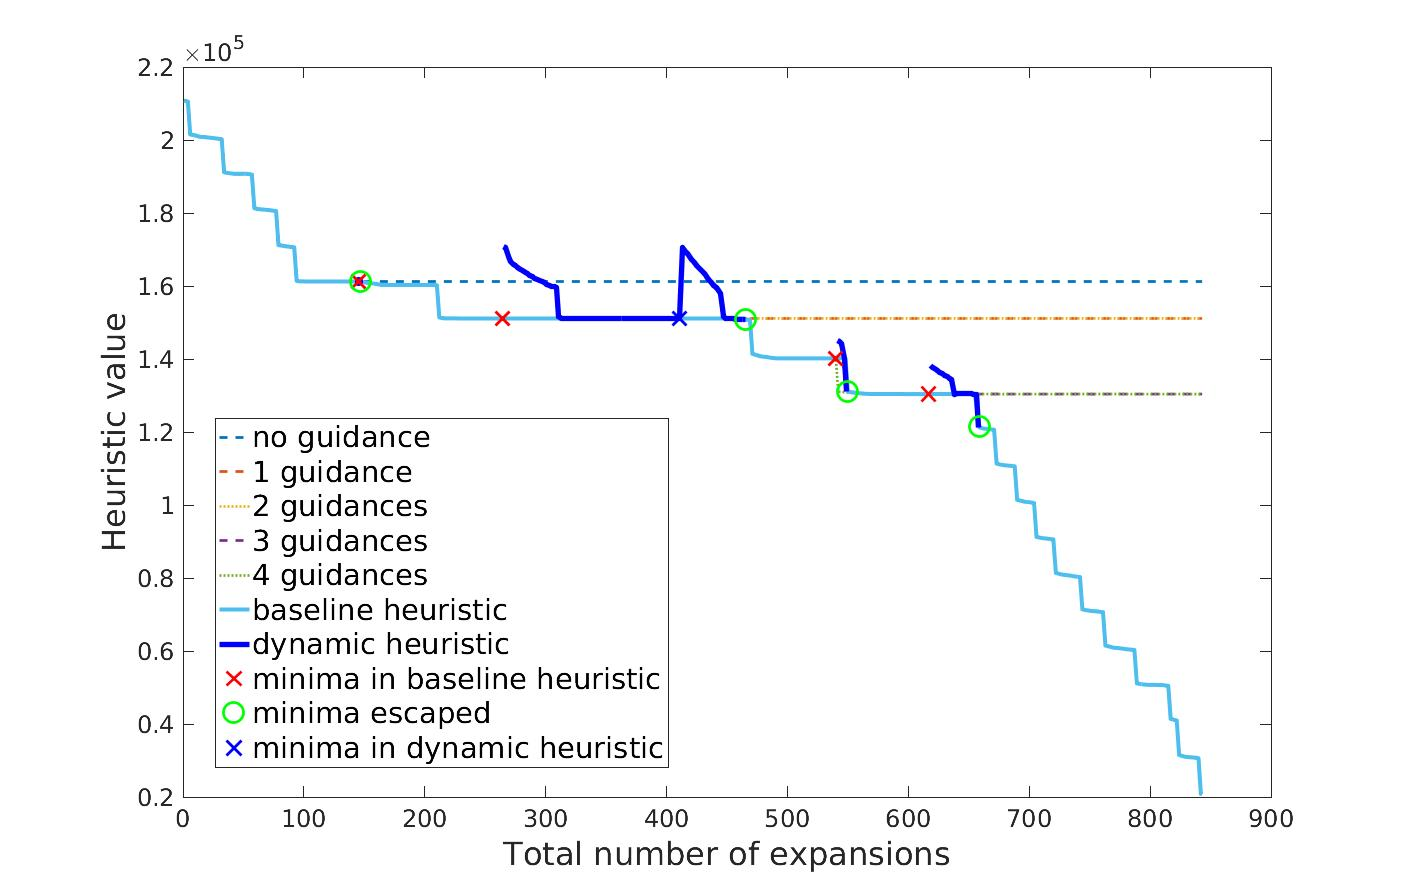
\includegraphics[width=0.4\textwidth]{heuristic_value.jpg}
  	\vspace{-2mm}
  \caption{
		Progress of MHA*---heuristic values as a function of the number of queue expansions.
		When a local minima is detected (red cross) in the baseline heuristic (cyan), a dynamic heuristic is generated (blue) until the local minima is escaped (green circle) or until a local minima is detected (blue cross) in the dynamic heuristic.
		Plots depicting the baseline heuristic values when only a limited amount of guidance is given demonstrate that without guidance, the planner remains stuck in local minima (we note that as MHA* is complete, it will eventually escape all local minima).
		}
\vspace{-5mm}
   	\label{fig:res}
\end{figure}

While providing promising initial results, our framework is far from being complete.
We are interested in experimenting with alternative forms of user guidance such as providing a \emph{constrained submanifold} of the configuration space. This may be used to guide the humanoid to use the railing while planning the stairs.
%Furthermore, we would like to have a \emph{recursive} implementation of our framework.
%Namely, the planner can be in a local minima while trying to escape a local minima. This should be identified and then the user should either (i)~provide new guidance 
%\os{This is already implemented}
%or 
%(ii)~provide  guidance  toward the previoulsy provided guidance.
Finally, once a guide is given, we want our planner to be able to \emph{generalize} the guidance obtained to future local minima that are similar in nature to the ones encountered.

%\newpage

%\bibliographystyle{plainnat}
\bibliographystyle{abbrv}
\bibliography{bibliography}

\end{document}

%%% Local Variables:
%%% mode: latex
%%% TeX-master: t
%%% End:
